\section{Related Work}
\label{s:related}

\textbf{RTS-CTS} There have been a variety of approaches to address the Hidden Terminal Problem. One approach, which is used in 
standard 802.11x protocols, utilizes a form of a feedback by having stations initiating a request-to-send (RTS) packet to the AP and having the AP respond to the station in the form of a clear-to-send (CTS) packet. The method 
mitigates the Hidden Terminal Problem because while the two terminals cannot sense each other, each can sense the clear to send frame from the AP. This is an indirect method to notify contending terminals that a transmission from some other terminals is about to begin. Once a contending terminal senses the CTS frame, it defer transmission and waits a random time interval called a backoff interval. The contending terminals then assess the channel again, and if the channel is clear, they transmit to the AP.  While the request-to-send/clear-to-send (RTS-CTS) protocol works in principal, in practice the additional messages that must be transmitted over the network to enable RTS-CTS significantly reduces the overall throughput.
	
\textbf{ARQ} Another well-known approach is automatic repeat request (ARQ). For this approach, if a packet loss occurs, the sender can either choose to adapt its transmission rate or retransmit the same packet again~\cite{80211_spec}. This choice typically depends on channel conditions. For a channel limited by the signal-to-noise ratio (SNR) of the link, adapting the rate will effectively decrease the packet loss because there is more energy per symbol. For other channels that have high SNR and sparse bursty traffic for which the co-channel interference is intermittent, it is more advantageous to use retransmissions. A key goal is to find the right balance between rate adaptation and retransmissions. 

\textbf{HARQ} For future networks that consist of many access points with intermittent co-channel interference,  researchers have investigated several retransmission techniques~\cite{hybridARQ} based on combining information in the original corrupted transmission with new information derived from the retransmitted packet. In one technique, called Chase Combining, every retransmission contains the same information. The receiver uses diversity combining to combine the received with the same bits from previous retransmissions. Because all transmissions are identical, Chase combining can be viewed as a form of repetition coding~\cite{chaseIR}. Alternatively, the technique of incremental redundancy involves sending a different block of information on each retransmission. Incidentally, RoXOR is closely related to the incremental redundancy approach of Hybrid ARQ. In the absence of an ACK from the AP, a RoXOR enabled STA iteratively sends incremental amounts of parity until the original corrupted packet is decoded successfully. What sets RoXOR apart from traditional incremental redundancy is the structure of the code used. RoXOR utilizes a rateless coding structure that is more suitable for contiguous bursts caused by co-channel interference.   

\begin{figure}[t]
\centering
\vspace*{-0.1in}
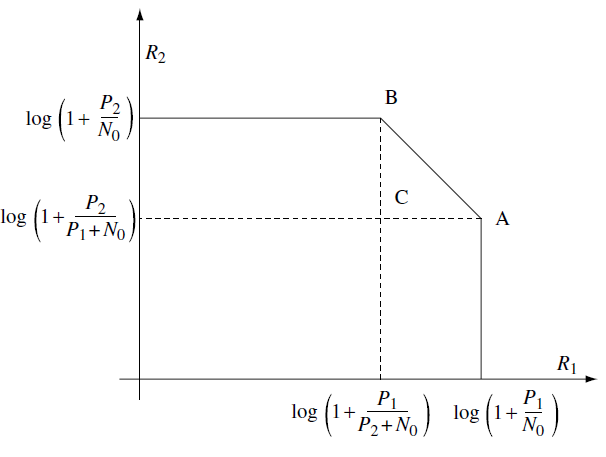
\includegraphics[width=.9\columnwidth]{./figs/mac.png}
\label{fig:mac}
\vskip -0.5em
\caption{Multiple Access Channel Capacity}
%\vskip -1em
\end{figure} 
 
\textbf{Multiple Access Channel} RoXOR also relies on results from multi-user information theory. Figure~\ref{fig:mac} shows the two user capacity region. When two-users wish to transmit on the same channel at the same time, their sum rate is limited to the feasible rate region within the pentagon. In order to obtain the optimal trade-off between the rates of the two users $R_1$ and $R_2$, indicated by points A and B, techniques such as successive interference cancellation must be applied~\cite{tse}.

\textbf{ZigZag} In essence, our work is inspired by ZigZag decoding. In the case of ZigZag, in the event of a packet error,  the STA retransmits the entire packet again and decodes both collided packets using successive interference cancellation~\cite{zigzag}. This strategy can be seen as a more conservative approach in the sense that, it probably wasn't necessary to send a whole packet's worth of redundancy to decode the corrupted packet. On the other hand, RoXOR differs from Zigzag because it only sends a coded fraction of the original packet. Furthermore, RoXOR can be seen as  a generalization of Zigzag, where the ``Zigzag'' encoder retransmits using code parameter $\beta=1$, which equates to re-transmitting the entirety of the original corrupted packet.

\textbf{SoftPHY} One component of SoftPHY~\cite{softphy} involves finding the corrupted portions of the original transmitted packet. Next, the SoftPHY enabled AP coordinates with the STA such that only the bits that were lost are re-transmitted back to the AP in hopes of successfully decoding the original packet. RoXOR avoids sending feedback and relies on the symmetry of its coding structure.
